% 设置编码,编码为UTF-8编码,字号大小12pt
\documentclass[UTF8, 12pt]{ctexart}
\usepackage{graphicx}
\usepackage{geometry}
\usepackage{titlesec}{\tiny}
\usepackage{amsmath}
\usepackage{authblk}
\usepackage{amsfonts}
\usepackage{url}
% 定义超链接的颜色
\usepackage[colorlinks, linkcolor=blue, citecolor=blue]{hyperref}

% 标题左对齐
%\CTEXsetup[format={\Large\bfseries}]{section}

% 定义
\newtheorem{theorem}{Theorem}[section]
% 控制图片的位置,让图片紧紧的跟住文字,只需写\begin{figure}[H]
\usepackage{float}
% 使用文献引用
\usepackage{cite}
% 使用算法排版模块
\usepackage{algorithm}  
\usepackage{algorithmic}
\renewcommand{\algorithmicrequire}{\textbf{输入:}}  
\renewcommand{\algorithmicensure}{\textbf{输出:}} 
% 设置文本格式,文本间距等,具体参考如下:
% left=2cm, right=2cm, top=2.5cm,bottom=1.5cm
\geometry{a4paper, centering, scale=0.8}
\newtheorem{thm}{定义}
\renewcommand{\baselinestretch}{1.3}

% 定义编程语言
\usepackage{listings}
\usepackage{color}
\usepackage{fontspec}
\definecolor{dkgreen}{rgb}{0,0.6,0}
\definecolor{gray}{rgb}{0.5,0.5,0.5}
\definecolor{mauve}{rgb}{0.58,0,0.82}
\definecolor{light-gray}{gray}{0.95}

\lstset{frame=tb,
		language=Python,
		aboveskip=3mm,
		belowskip=1mm,
		showstringspaces=false,
		columns=flexible,
		basicstyle=\small\ttfamily,
		numbers=left,
		numberstyle=\small\color{gray},
		keywordstyle=\color{blue},
		commentstyle=\color{dkgreen},
		stringstyle=\color{mauve},
		breaklines=true,
		breakatwhitespace=true,
		tabsize=4,
		backgroundcolor=\color{light-gray}
}

\begin{document}

	
	\title{\heiti \Huge{GloVe: Global Vectors for Word Representation}}
	\author{\kaishu 尹卓 \\ E-mails: \href{mailto:zhuoyin94@163.com}{zhuoyin94@163.com}}
	\date{\today}
	\maketitle
	
	% 增加目录
	\tableofcontents
	\newpage
	\section{Abstract与Related Work简介}
	本文\cite{pennington2014glove}设计了一种新的全局对数双线性回归模型(Global Log-bilinear Regression Model)对词的进行向量化编码表示的方法,该方法结合了两种主要模型的优点:一种是基于全局矩阵分解的方法,另一种是基于局部滑窗的方法。对词的向量化工作,主要分为两种类型的工作:
	\begin{enumerate}
		\item \textbf{基于矩阵分解的方法(Matrix Factorization Methods)}:使用低秩近似(Low-Rank Approximations)的方法对能够捕获语料统计信息的大矩阵进行分解,构建矩阵的方法和形式多种多样,典型的方法是LSA相关的一系列工作。
		\item \textbf{基于粗略滑窗的方法(Shallow Window-Based Methods)}:利用模型通过预测滑窗内部的局部内容的方式,学习词向量的表示,典型的是Word2Vec相关的工作。
	\end{enumerate}

	\section{GloVe模型原理}
	大语料中词语之间共现性的统计特性是词向量表示学习中最主要的想要学习到的目标。假设词与词的共现性矩阵:$X$,其中$X_{ij}$代表了第$j$词出现在第$i$词指定窗口大小中的次数。$X_{i} = \sum_{k}X_{ik}$为任何词出现在词$i$中的附近次数之和。设$P_{ij} = P(j|i) = X_{ij}/X_{i}$表示第$j$词出现在中心词$i$窗口内的概率。

	\begin{figure}[H]
		\centering
		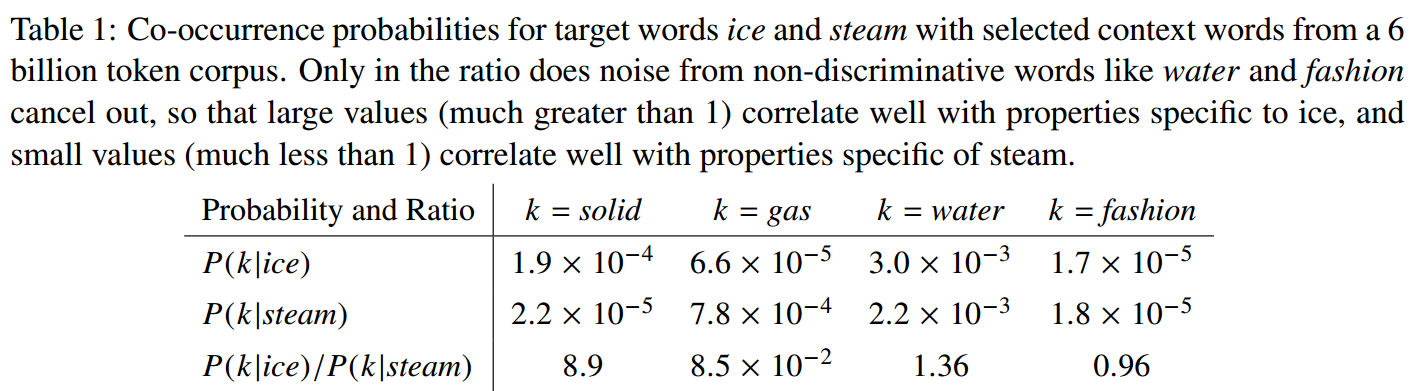
\includegraphics[width=0.85\linewidth]{..//Plots//table_1.png}
		\caption{共现矩阵示意}
		\label{tab_1}
		\vspace{-0.5em}
	\end{figure}

	由表(\ref{tab_1})可知,因为词的共现性矩阵能够一定程度上反映语料中词与词之间的统计特性,因此对共现矩阵的处理也许是词向量化的一个好的起点。所以可以先假设:
	\begin{equation}
		F(w_{i}, w_{j}, \tilde{w}_{k}) = \frac{P_{ik}}{P_{jk}}
	\end{equation}
	其中$w \in \mathbb{R}^{d}$为词的向量表示,$\tilde{w}_{k}$的作用可参见后续步骤。式子中$F$函数应当满足一些条件:首先$F$可以编码$P_{ik}/P_{jk}$的信息,所以$F$表达式应该融入$w_{i}$与$w_{j}$向量的信息,其中向量加减法是最自然的方法。因此可设:
	\begin{equation}
		F(w_{i} - w_{j}, \tilde{w}_{k}) = \frac{P_{ik}}{P_{jk}}
	\end{equation}
	其次,我们注意到上式中等号右边为标量,因此我们采取向量点乘的方法保持等号一致性:
	\begin{equation}
		F((w_{i} - w_{j})^{T}\tilde{w}_{k}) = \frac{P_{ik}}{P_{jk}}
	\end{equation}
	然后又注意到,对于共现矩阵而言具有对称性,也就是词与中心词角色可以任意互换。因此我们的模型应该具有对称性。而这个对称性可以由以下一系列步骤来保证:
	\begin{equation}
		F((w_{i} - w_{j})^{T}\tilde{w}_{k}) = \frac{F(w_{i}^{T}\tilde{w}_{k})}{F(w_{j}^{T}\tilde{w}_{k})}
	\end{equation}
	其中:
	\begin{equation}
		F(w_{i}^{T}\tilde{w}_{k}) = P_{ik} = \frac{X_{ik}}{X_{i}}
	\end{equation}
	使得$F = exp$的话:
	\begin{equation}
		w_{i}^{T}\tilde{w}_{k} = log(X_{ik}) - log(X_{i})
	\end{equation}
	注意到上式中,因为$X_{i}$出现在等式右边,所以该式子等号两边不是对称的。但是由于该项是与$k$无关的,可以作为参数吸收进$b_{i}$,因此:
	\begin{equation}
		w_{i}^{T}\tilde{w}_{k} + b_{i} + \tilde{b}_{k} = log(X_{ik})
	\end{equation}
	这样就维持了整体表达式的等价性。事实上$\tilde{w}_{k}$与$\tilde{b}_{k}$是作为某种形式的参数出现在式子里。以上模型最为显著的缺点是将每一个词的视为同等的重要。

	对于上面的式子的优化,作者提出使用加权线性回归(Weighted Least Squares Regreesion Model)的方法来解:
	\begin{equation}
		J = \sum_{i, j = 1}^{V} f(X_{ij}) (w_{i}^{T}\tilde{w}_{j} + b_{i} + \tilde{b}_{j} - log(X_{ij}))^2
		\label{glove_loss}
	\end{equation}
	其中$V$为词表大小。这个加权线性回归的加权函数$f$应该有如下几个特性:
	\begin{enumerate}
		\item $f(0) = 0$。如果两个单词没有出现过共现性,那自然权重应该为0。
		\item $f(x)$应当是非递减的(Non-decreasing),因此非常罕见的共现词不会过分被加权。
		\item $f(x)$对于$x$比较大的时候应该相对较小,这样频繁出现的共现词不会过分被加权。
	\end{enumerate}
	因此作者选用以下加权函数:
	\begin{equation}
	f(x) = 
		\begin{cases}
			(x / x_{max})^{\alpha}; & if \; x < x_{max} \\
			1; & otherwise
		\end{cases}
	\end{equation}
	其中作者设置$x_{max} = 100$,并且通过实验发现$\alpha = 3/4$能够取得最好的效果,如图(\ref{fig_1})为加权函数的图像。

	\begin{figure}[H]
		\centering
		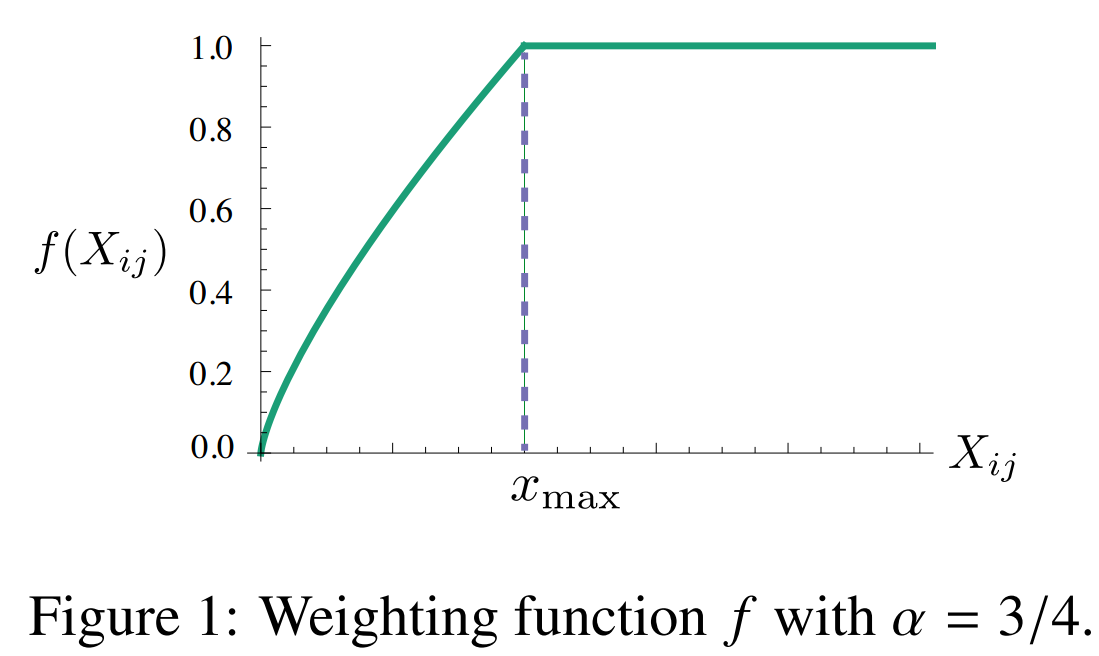
\includegraphics[width=0.45\linewidth]{..//Plots//fig_1.png}
		\caption{加权函数图像}
		\label{fig_1}
		\vspace{-0.5em}
	\end{figure}

	\section{GloVe模型与SkipGram模型的联系}
	由于词向量学习的模型多多少少都基于共现矩阵的性质,因此作者主要对Skip-Gram与GloVe的区别进行了对比。对于Skip-Gram模型而言,模型希望建模词$j$出现在中心词$i$窗口中的概率。假设$Q_{ij}$为softmax函数,并且有如下的形式:
	\begin{equation}
		Q_{ij}  = \frac{exp(w_{i}^{T}\tilde{w}_{j})}{\sum_{k=1}^{V}exp(w_{i}^{T}\tilde{w}_{k})}
	\end{equation}
	对于Skip-Gram的全局目标函数(Global Objective Function)可以被写作:
	\begin{equation}
		J = - \sum_{i \in corpus \atop j \in context(i)} \log Q_{ij}
	\end{equation}
	由于上式每项规范化因子计算量太大,Skip-Gram模型一般选择近似计算$Q_{ij}$。不过对于上式而言,我们可以实现做这样的操作提升计算效率:
	\begin{equation}
		J = -\sum_{i=1}^{V}\sum_{j=1}^{V}X_{ij}\log Q_{ij}
	\end{equation}
	这样避免了一些重复的计算。之前定义$X_{i} = \sum_{k}X_{ik}$以及$P_{ij} = X_{ij} / X_{i}$,因此我们可以重写$J$为:
	\begin{equation}
		J = - \sum_{i=1}^{V}X_{i}\sum_{j=1}^{V}P_{ij}\log Q_{ij}=\sum_{i=1}^{V}X_{i}H(P_{i}, Q_{i})
		\label{sg_loss}
	\end{equation}
	其中$H(P_{i}, Q_{i})$是分布$P_{i}$与分布$Q_{i}$的交叉熵。事实上式(\ref{sg_loss})与式(\ref{glove_loss})是有一定的相似性的。由于式(\ref{sg_loss})采用了交叉熵,因此计算规范化因子需要遍历词表,更好的方式是采用最小二乘(Least Square)的方式直接避免计算归一化因子:
	\begin{equation}
		\hat{J}= \sum_{i,j}X_{i}(\hat{P}_{ij} - \hat{Q}_{ij})^{2}
	\end{equation}
	其中$\hat{P}_{ij} = X_{ij}$,$\hat{Q}_{ij} = exp(w_{i}^{T}\tilde{w}_{j})$。在这个式子中,又存在其他的问题:$X_{ij}$可以取非常大的值,使得优化方法不稳定。比较有效的补救方法是采用对数来进行约束:
	\begin{align}
		\hat{J} & = \sum_{i,j}X_{i}(\log \hat{P}_{ij} - \log \hat{Q}_{ij})^{2} \\
				& = \sum_{i,j}X_{i}(w_{i}^{T}\tilde{w}_{j} - \log X_{ij})^{2}
	\end{align}
	最后,我们可以观察到$X_{i}$在该式子中扮演了(\ref{glove_loss})中权值的角色,事实上Mikolov et al.\cite{mikolov2013distributed}观察到通过控制每个词的词频可以起到提升模型表现的效果。因此上式可以被改写为:
	\begin{equation}
		\sum_{i,j}f(X_{i})(w_{i}^{T}\tilde{w}_{j} - \log X_{ij})^{2}
	\end{equation}
	这就形成了Skip-Gram模型与GloVe模型(\ref{glove_loss})形式上的一致性。试验结果分析可参见原文\cite{pennington2014glove}与博客\cite{范永勇},更优秀的Tutorial参见\cite{hans}。

	\bibliographystyle{unsrt}
	\bibliography{GloVe_ref}
\end{document}